\chapter{Cơ sở lý thuyết}


% \subsection{\texorpdfstring{Trí tuệ nhân tạo, học máy và học sâu}{ai_ml_dl}}

% Định nghĩa:
% \begin{itemize}
%     \item \textbf{Trí tuệ nhân tạo:} Là ngành nghiên cứu về cách thực hiện các chương trình máy tính có khả năng mô phỏng suy nghĩ và khả năng giải quyết vấn đề ở cấp độ con người
%     \item \textbf{Học máy:} Là tập con của ngành trí tuệ nhân tạo, là ngành nghiên cứu cách thực hiện các chương trình máy tính mà không phải có mã lập trình tường minh, có chức năng tự động học các tri thức của con người để cải thiện các quyết định của nó trên các dữ liệu mà nó chưa từng gặp trước đây.
%     \item \textbf{Học sâu:} Là tập con của ngành học máy, là tập hợp các giải thuật học máy có sử dụng mạng thần kinh nhân tạo có cấu trúc tương tự mạng thần kinh trong não bộ con người để học cách đưa ra quyết định.
% \end{itemize}

% \begin{figure}[H]
%     \centering
%     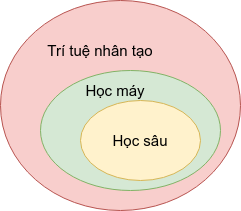
\includegraphics[width=7cm]{./content/materials/ai_ml_dl.png}
%     \caption{Trí tuệ nhân tạo, học máy và học sâu}
% \end{figure}


% Ngày nay, ngành học máy và học sâu ngày càng chiếm nhiều ưu thế so với các phương pháp khác trong các ứng dụng thực tế do có độ tổng quát dữ liệu tốt, độ chính xác cao, và có thể mô hình hóa các vấn đề phức tạp, trừu tượng trong đời sống. Đối với các vấn đề phức tạp như thị giác máy, dịch máy, đánh nhãn văn bản tự động, tạo sinh dữ liệu,... các giải thuật học sâu luôn là lựa chọn hoàn hảo do nó có khả năng tổng quát hóa một lượng dữ liệu rất lớn. Một lợi điểm khác của việc sử dụng các giải thuật học sâu là các giải thuật này có khả năng tìm ra các đặc trưng của dữ liệu một cách tự động. Trong khi các giải thuật học máy truyền thống chỉ có khả năng xử lý tốt trên dữ liệu đã được rút trích đặc trưng bằng các giải thuật xử lý dữ liệu truyền thống, các mạng học sâu có khả năng tự học lấy các đặc trưng của dữ liệu. Tuy nhiên, các giải thuật học sâu yêu cầu một lượng dữ liệu lớn để học. Bên cạnh đó, bài toán phải được mô hình hóa hợp lý, mạng thần kinh học sâu cũng phải được thiết kế phù hợp với mô hình bài toán để khiến cho việc học của mạng thần kinh dễ dàng và hiệu quả hơn.

% \subsection{\texorpdfstring{Tính chất tổng quát hóa dữ liệu của mạng thần kinh học sâu}{dl_network}}
% Mạng thần kinh học sâu có khả năng tổng quát hóa dữ liệu cao, nhờ vào đó, nó có thể được huấn luyện để học bất cứ thứ gì nếu nó được mô hình hóa một cách hợp lý. Một mạng học sâu đạt được mức độ tổng quát hóa dữ liệu cao bằng cách học những đặc trưng ẩn của dữ liệu được dùng để huấn luyện nó. Vì vậy, mạng học sâu có thể đưa ra dự đoán trên những dữ liệu mới mà nó chưa từng nhìn thấy nhờ vào việc nội suy, nhưng những dữ liệu đó phải tương tự với dữ liệu được dùng để huấn luyện nó. Với những dữ liệu nằm ngoài phân phối dữ liệu huấn luyện, mạng thần kinh học sâu sẽ không có khả năng đưa ra kết quả chính xác bởi cấu trúc và các thông số trong mạng thần kinh không được điều chỉnh đề phù hợp với những dữ liệu đó.

\section{\texorpdfstring{Các cấu trúc trong mạng học sâu được sử dụng trong luận văn}{dl_basic_structures}}

% \subsection{Mạng thần kinh tích chập (Convolution)}
% Trước khi có mạng học sâu, việc trích xuất đặc trưng bằng các kĩ thuật đặc biệt cho từng loại dữ liệu khác nhau là công đoạn quan trọng nhất trong quá trình giải quyết một bài toán. Lý do là bởi mạng thần kinh truyền thống không có khả năng tạo ra các chiều không gian đủ rộng để tự học các đặc trưng của dữ liệu. Thông thường, phép tích chập được thực hiện bằng các nhân tích chập (kernel). Một phép tích chập được đặc trưng bởi số lượng kênh đầu vào, số lượng kênh đầu ra và kích thước của nhân tích chập.

% \begin{figure}[H]
%     \centering
%     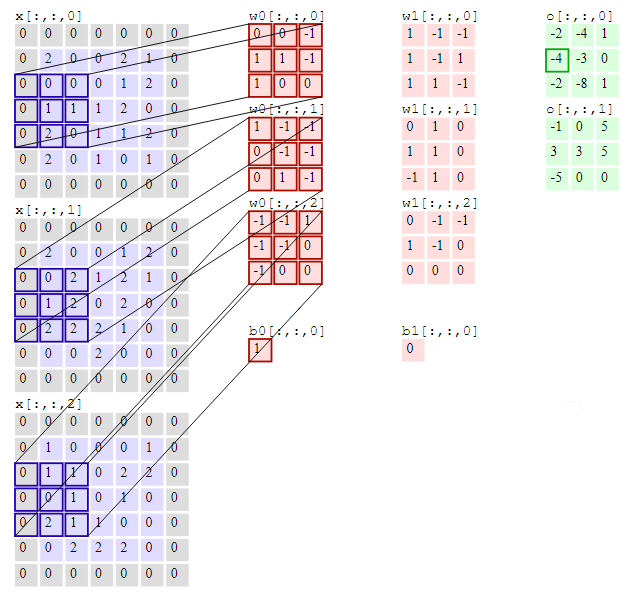
\includegraphics[width=15cm]{./content/materials/cnn.png}
%     \caption{Cách tính tích chập. Nguồn: Internet}
% \end{figure}

% Ví dụ, một phép tích chập với nhân có kích thước $m$x$m$ được thực hiện trên một ma trận ba chiều kích thước $H$x$H$x$K$ sẽ cho ta một ma trận kết quả có kích thước $(N-m+1)$x$(N-m+1)$
% Phép tích chập cho ma trận hai chiều trong mạng được biểu diễn bởi phương trình sau:

% \begin{equation}
%     o_{ijm}=\sum_{k=0}^{K-1}\sum_{p=0}^{H-1}\sum_{q=0}^{H-1}x_{i+p,j+q,k}^{(l-1)}w_{pqkm}+b_{ijm}
% \end{equation}

% Sự xuất hiện của mạng thần kinh tích chập đã giúp cho việc trích xuất đặc trưng trở nên dễ dàng hơn và đôi khi là không cần thiết nhờ vào khả năng tự động trích xuất đặc trưng của mạng. Sở dĩ mạng thần kinh tích chập có khả năng trích xuất đặc trưng tốt là nhờ vào việc nó tập trung vào học các kiễu mẫu rất chi tiết hay xuất hiện trong dữ liệu ở các lớp đầu. Ở các lớp sau, những tri thức học được càng được tổng quát dần bằng việc kết hợp các tri thức học được từ lớp trước vào tạo nên những hiểu biết ở bậc cao nhất của dữ liệu ở các lớp tích chập cuối cùng.

% Nhưng điều này không có nghĩa là chỉ cần sử dụng mạng thần kinh tích chập thì ta sẽ không cần quan tâm tới việc trích xuất đặc trưng nữa bởi khi có những đặc trưng tốt được đưa vào mạng, mạng tích chập vẫn cho ra kết quả tốt hơn, chính xác hơn với ít dữ liệu hơn và thời gian huấn luyện cũng nhanh hơn. Ngoài ra, lớp tích chập cũng có số lượng hệ số học nhỏ, huấn luyện nhanh, vì vậy nó hay được đặt nằm ở các lớp đầu và giữa trong các mạng học sâu để trích xuất dữ liệu nhanh và hiệu quả hơn.

\subsection{Tích chập ngược (Deconvolution) \cite{deconv}}

Mạng tích chập ngược có tính năng ngược với mạng tích chập truyền thống. Nếu như mạng tích chập có chức năng mã hóa, rút trích đặc trưng của dữ liệu đầu vào, thì mạng tích chập ngược nhận vào những đặc trưng đã được rút trích của dữ liệu và tạo sinh ngược lại dữ liệu với cấu trức tương tự ban đầu. Phép tích chập ngược cũng được đặc trưng bởi kích thước nhân, số lượng kênh đầu vào và đầu ra, bước nhảy của nhân tích chập ngược trên dữ liệu.

Phép tích chập ngược thường hay được sử dụng để tái thiết lập lại cấu trúc ban đầu. Thay vì rút trích và thu nhỏ dữ liệu ban đầu thành những đặc trưng như mạng tích chập, mạng tích chập ngược sử dụng các đặc trưng đã được rút trích và học các trọng số để tạo ra dữ liệu mới có cấu trúc giống với dữ liệu được trích xuất đặc trưng ban đầu. Vì vậy, mạng tích chập ngược có tính năng tạo sinh dữ liệu và hay được sử dụng trong các ứng dụng như:

\begin{itemize}
    \item \textbf{Autoencoder \cite{autoencoder}:} Cấu trúc của một Autoencoder bao gồm một mạng tích chập và một mạng tích chập ngược ghép nối tiếp với nhau. Mạng tích chập có chức năng thu nhỏ và rút trích đặc trưng từ dữ liệu gốc. Trong khi đó, một mạng tích chập ngược dùng véc tơ đặc trưng vừa được tạo ra bởi mạng tích chập để cố gắng tái tạo lại dữ liệu gốc.
    \item \textbf{Hệ thống phân đoạn ảnh \cite{img_segmentation}:} Hệ thống phân đoạn hình ảnh có chức năng đánh nhãn cho từng điểm ảnh để xem nó thuộc vào lớp nào. Sau khi rút trích đặc trưng từ ảnh, mạng tích chập ngược được dùng để biên dịch đặc trưng ảnh thành mặt nạ phân lớp cho ảnh.
    \item \textbf{Variational Autoencoder \cite{vae_base}:} Đây là một loại mạng nơ ron dùng để tạo sinh dữ liệu dựa trên phân phối xác suất mà nó học được từ dữ liệu mẫu. Với phân phối xác suất học được, mạng có thể tạo ra được dữ liệu có tính chất, cấu trúc tương tự như dữ liệu mẫu nhưng chưa từng tồn tại trong dữ liệu mẫu. Ví dụ: cho mạng Variational Autoencoder học cách tạo sinh hình ảnh của các chữ số trong tập MNIST, sau đây là ảnh được tạo sinh: 
        \begin{figure}[H]
            \centering
            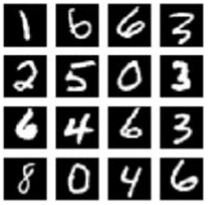
\includegraphics[width=7cm]{./content/materials/mnist_vae.png}
            \caption{Tạo sinh ảnh cùng phân phối xác suất với tập dữ liệu MNIST}
        \end{figure}
    \item \textbf{Mạng GANs (Generative Adversarial Networks) \cite{gans_base}:} Là một loại mạng tạo sinh dữ liệu bằng cách học cấu trúc dữ liệu của các mẫu dữ liệu được dùng để huấn luyện. Tùy thuộc vào tiêu chí được cài đặt, mạng GANs sẽ sinh ra dữ liệu cố gắng thỏa mãn tiêu chí được yêu cầu. Đây cũng là cấu trúc mạng được dùng trong luận văn.
\end{itemize}

% \subsubsection{Lớp kết nối đầy đủ (Fully Connected)}
% Lớp kết nối đầy đủ là lớp chính của mạng nơ ron truyền thống và được xem là một phép biến đổi tuyến tính trong mạng học sâu với phương trình:
% \begin{equation}
%     y=xA^T+b
% \end{equation}
% Với phương trình trên, lớp kết nối đầy đủ là một mạng lưới perceptron đơn lớp, với:
% \begin{itemize}
%     \item Đầu vào là véc tơ $x$ với $N_x$ chiều
%     \item Đầu ra là véc tơ $y$ với $N_y$ chiều
%     \item Véc tơ $b$ có $N_y$ chiều
%     \item $A$ là ma trận có kích thước $N_y$x$N_x$
% \end{itemize}
% Trong mạng học sâu, lớp kết nối đầy đủ thường được đặt ở vị trí sâu nhất của mạng để thực hiện biến đổi tuyến tính cuối cùng từ những đặc trưng được trích xuất từ các lớp trước đó để cho ra kết quả cuối cùng nhờ vào khả năng học những đặc trưng tổng quát. Tuy nhiên, đây không phải là lớp biến đổi dữ liệu có khả năng học được các đặc trưng dữ liệu ở mức độ chi tiết như mạng tích chập, có số lượng trọng số học lớn và chỉ đặc trưng duy nhất cho một bài toán, không thể tái sử dụng lại cho bài toán khác.

\subsection{Mạng nơ ron hồi quy (RNN)}

Trong cuộc sống hằng ngày, đôi khi ta phải xử lý các loại dữ liệu có tính chất chuỗi, đó là các dữ liệu có tính trật tự. Khác với kiểu dữ liệu truyền thống khi mà các mẫu dữ liệu không có tính chất chuỗi, không có thứ tự và độc lập lẫn nhau, đối với dữ liệu chuỗi, thứ tự của các mẫu dữ liệu là quan trọng và mang ý nghĩa nhất định. Nếu thứ tự này bị thay đổi thì dữ liệu bị mất đi hoàn toàn tính chất, thông tin mà nó mang lại. Một số ví dụ về thông tin dạng chuỗi có thể liệt kê như: ngôn ngữ tự nhiên, dữ liệu có đặc tính thời gian như nhiệt độ trong ngày, giá chứng khoán, dữ liệu âm thanh và video. Dữ liệu chuỗi còn có một đặc tính khác biệt so với các dữ liệu truyền thống là nó có độ dài bất định, một câu có thể có nhiều từ ngữ, đoạn âm thanh hay video có thể có độ dài dài ngắn khác nhau. 

Tuy nhiên, mạng tích chập (CNN) và mạng kết nối đầy đủ (Fully Connected) được thiết kế theo kiểu đường thẳng (feed-forward), nhằm mục đích tạo ra kết quả đầu ra chỉ dựa trên đầu vào (không có đường nối vòng trên đồ thị tính toán). Nhưng đối với dữ liệu chuỗi, đầu ra $y_i$ bất kì tại vị trí $i$ không chỉ phụ thuộc vào đầu vào $x_i$, mà nó còn phụ thuộc vào những mẫu dữ liệu đến trước $x_i$ ($x_{i-1}$, $x_{i-2}$, ...) cũng như thứ tự của chúng trong đầu vào, và đôi khi hoàn toàn không phụ thuộc vào các mẫu dữ liệu đến sau ($x_{i+1}$, $x_{i+2}$, ...). Do đó, các cấu trúc mạng theo kiểu đường thẳng đôi khi không thể dùng được cho bài toán dữ liệu chuỗi, điều này dẫn đến sự ra đời của mạng nơ ron hồi quy.

Mạng nơ ron hồi quy (Recurrent Neural Networks - RNN) là một kiến trúc mạng học sâu mà trong đó trạng thái của các bước trước sẽ được dùng như một đầu vào của bước sau. Với RNN, thông tin được xử lý tuần tự theo thứ tự trong chuỗi. Do việc sử dụng trạng thái ẩn của bước trước cho bước sau, mạng RNN tạo ra một đường vòng trên đồ thị tính toán. Nói cách khác, trạng thái ẩn đóng vai trò như một bộ nhớ tạm thời trong RNN, điều này làm cho việc xử lý dữ liệu dạng chuỗi bằng RNN trở nên hiệu quả hơn hẳn so với các phương pháp cũ. Hình sau thể hiện cấu trúc tính toán của mạng RNN:

\begin{figure}[H]
    \centering
    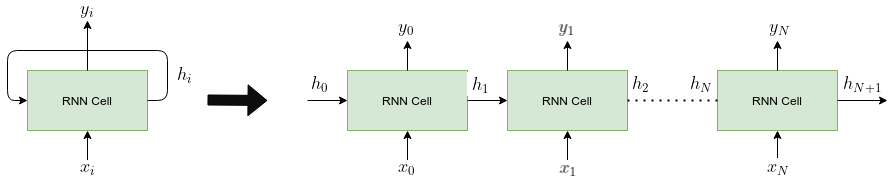
\includegraphics[width=15cm]{./content/materials/rnns.png}
    \caption{Cấu trúc tính toán của RNN}
\end{figure}

Công thức truy hồi của mạng hồi quy RNN được biểu diễn như sau:

\begin{equation}
\begin{split}
    &h_0=0\\
    &h_i=f(W_{hx}*x_i+W_{hh}*h_{i-1}+b_h)\\
    &y_i=g(W_{yh}*hi+b_y)\\
\end{split}
\end{equation}

Với:
\begin{itemize}
    \item \textbf{$h_i$:} Trạng thái ẩn ở bước thứ i
    \item \textbf{$x_i$:} Đầu vào của mạng ở bước thứ i
    \item \textbf{$y_i$:} Đầu ra của mạng ở bước thứ i
    \item \textbf{$W_{hx}$, $W_{hh}$, $W_{yh}$ và $b_h$, $b_y$:} Các trọng số của mạng 
\end{itemize}

Về lý thuyết, mỗi đầu vào của mạng RNN đều cho ra một kết quả ở đầu ra và tạo ra một trạng thái mới cho mạng, sử dụng các kết quả tính toán này như thế nào là tùy vào cách mô hình hóa bài toán và mục tiêu của bài toán. Việc xác định sử dụng kết quả ở đầu ra nào là rất quan trọng vì trọng số của mạng sẽ được cập nhật dựa vào kết quả đó.

Tóm lại, RNN được thiết kế đặc thù cho việc giải quyết dữ liệu dạng chuỗi, với ưu điểm là có khả năng giải quyết chuỗi với độ dài bất định với kích thước mô hình cố định, không phụ thuộc vào đầu vào. Việc tính toán của mạng RNN có xem xét tới thông tin ở quá khứ và chia sẻ trong số trong quá trình tính toán giúp cho mạng giảm số lượng trọng số học và cải thiện tính tổng quát hóa, tránh tình trạng học thuộc. Tuy nhiên, do việc tính toán diễn ra tuần tự nên việc tính toán song song bị hạn chế. Đồng thời RNN cũng có khả năng bị "quên" mất dữ liệu được học trước đó nếu chuỗi dữ liệu quá dài.

% \subsubsection{Lớp lấy mẫu (Pooling)}

% Lớp lấy mẫu thường được sử dụng khi chúng ta muốn giảm bớt kích thước của dữ liệu nhưng vẫn giữ được những đặc trưng nổi bật nhất. Lớp lấy mẫu dùng một cửa sổ thường có kích thước hình vuông $m$x$m$ (thuờng được chọn là 2x2) để quét qua tất cả các ô trên ma trận dữ liệu kích thước $N$x$N$ và thực hiện phép lấy mẫu trên cửa sổ đó. Kết quả cuối cùng sẽ là ma trận có kích thước $\frac{N}{m}$x$\frac{N}{m}$. Tùy vào phép lấy mẫu nào được thực hiện mà kết quả của mỗi lần lấy mẫu sẽ khác nhau. Có hai phép lấy mẫu thường được sử dụng là lấy mẫu lớn nhất (Max Pooling) và lấy mẫu trung bình (Average Pooling). Trong đó, phép lấy mẫu lớn nhất thường được sử dụng để lấy ra đặc trưng nổi bật nhất của dữ liệu, trong khi phép lấy mẫu trung bình thường được dùng để thu nhỏ dữ liệu và trung hòa các đặc trưng xung quanh. Tùy vào mục đích cuối cùng của mạng mà sử dụng phép lấy mẫu sao cho hợp lý.

% \begin{figure}[H]
%     \centering
%     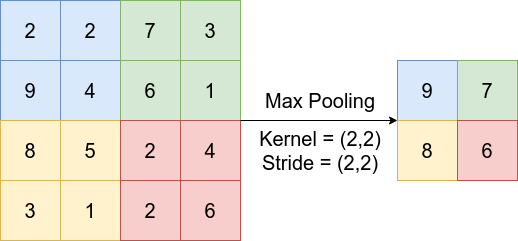
\includegraphics[width=10cm]{./content/materials/max_pooling.png}
%     \caption{Ví dụ tính toán lớp lấy mẫu lớn nhất (Max Pooling)}
% \end{figure}

\subsection{Lớp chuẩn hóa theo bó (Batchnorm)}

Việc huấn luyện mạng học sâu có chiều sâu lớn thường rất khó khăn do càng đi sâu vào mạng, gradient của các trọng số càng giảm và đôi khi tiến rất gần về 0. Do đó, lúc cập nhật trọng số, do gradient xấp xỉ 0 nên trọng số không được cập nhật và điều chỉnh nhiều. Đồng thời, khi huấn luyện mạng, các lớp trong mạng được cập nhật trọng số mà không quan tâm tới sự thay đổi trọng số của các lớp trước nó, và sự thay đổi trọng số này được thực hiện với giả sử là trọng số các lớp trước được giữ nguyên. Nhưng trên thực tế, các trọng số trong tất cả các lớp đều được cập nhật trong quá trình huấn luyện. Vì vậy, lớp chuẩn hóa theo bó được ra đời nhằm mục đích chuẩn hóa đầu ra của các lớp trước nó, nhờ vậy, các lớp phía sau sẽ nhận được đầu vào là các ma trận đã được chuẩn hóa, có giá trị trung bình bằng 0 và độ lệch chuẩn bằng 1 (phân phối Gaussian chuẩn). Việc chuẩn hóa này làm cho việc huấn luyện mạng trở nên ổn định hơn, hạn chế tình trạng triệt tiêu gradient và đẩy quá trình huấn luyện nhanh hơn nhiều lần

\begin{figure}[H]
    \centering
    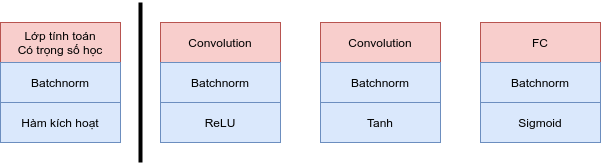
\includegraphics[width=13cm]{./content/materials/batchnorm.png}
    \caption{Một số cách đặt Batchnorm phổ biến}
\end{figure}

Hình trên miêu tả những cách đặt lớp chuẩn hóa theo bó phổ biến. Lớp chuẩn hóa theo bó thường được đặt sau một lớp tính toán có trọng số, nhờ đó, khi trọng số của lớp tính toán này được cập nhật và thay đổi, lớp Batchnorm sẽ chuẩn hóa kết quả này, nhờ đó, các lớp sau sẽ nhận được các tín hiệu có phân phối không thay đổi nhiều. Cũng nhờ vậy mà các hàm kích hoạt cũng hoạt động hiệu quả hơn. Do lớp Batchnorm cố gắng chuẩn hóa phân phối xác suất của đầu vào sao cho đầu ra của nó là một phân phối chuẩn có giá trị trung bình bằng 0 và phương sai bằng 1, và các hàm kích hoạt như ReLU, Tanh, Sigmoid đều có điểm cắt tại 0, nên gần như một nửa đầu vào của hàm kích hoạt sẽ nhỏ hơn 0 và nửa còn lại sẽ lớn hơn 0, do đó khi áp dụng các hàm kích hoạt cho phân phối này, các hàm kích hoạt sẽ đạt hiệu quả cao nhất.

\subsection{Mạng nơ ron hồi quy tích chập (CRNN)}

Trong xử lý hình ảnh, người ta thường dùng mạng tích chập (CNN), nhưng đối với video là một chuỗi hình ảnh theo thời gian, ta phải xem xét tính chất thay đổi theo thời gian của hình ảnh. Vì vậy, việc sử dụng kết hợp mạng tích chập (CNN) và mạng hồi quy (RNN) tạo ra mạng hồi quy tích chập (CRNN) được dùng để xử lý các dạng dữ liệu theo chuỗi thời gian với phương pháp tích chập. Mạng nơ ron hồi quy tích chập gồm hai phần chính:

\begin{itemize}
    \item \textbf{Mạng tích chập:} Mạng tích chập sử dụng mạng CNN để rút trích đặc trưng từ dữ liệu được đưa vào mạng. Các lớp được sử dụng trong mạng này bao gồm lớp tích chập, lớp lấy mẫu (Pooling) và lớp chuẩn hóa theo bó (Batchnorm). Theo đó, mạng này rút trích đặc trưng nhờ vào phép tích chập và sắp xếp các đặc trưng này thành chuỗi các đặc trưng có tính chất liên tục theo thời gian.
    \item \textbf{Mạng hồi quy:} Mạng hồi quy thường được sử dụng là LSTM hai hướng (Bidirectional-LSTM) và có thể có nhiều lớp hồi quy. Tại đây, các đặc trưng được rút trích từ mạng tích chập được đưa vào mạng theo tuần tự.
\end{itemize}

\begin{figure}[H]
    \centering
    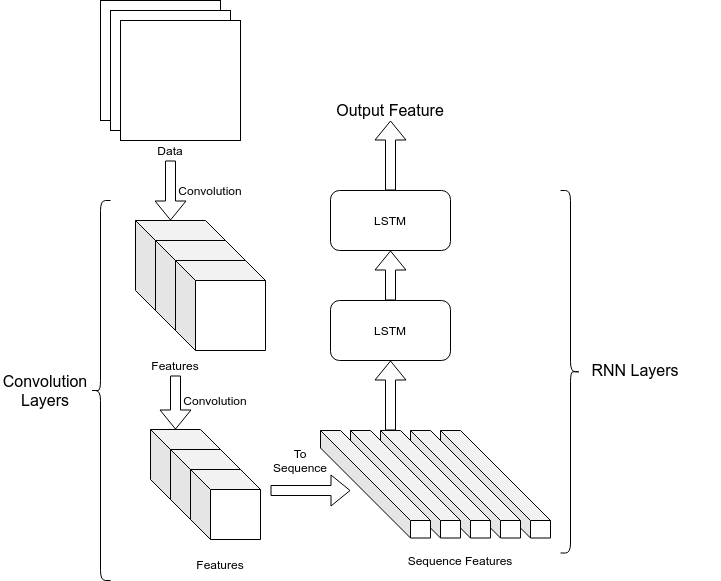
\includegraphics[width=13cm]{./content/materials/crnn.png}
    \caption{Ví dụ về mạng hồi quy tích chập CRNN}
\end{figure}

Ở đầu ra, các đặc trưng sau khi qua mạng hồi quy được sử dụng để đưa ra dự đoán. Cách sử dụng các đặc trưng này tùy thuộc vào yêu cầu của bài toán (tương tự như mạng RNN).

\subsection{Mạng nơ ron nối tắt (Residual Network)}

Về mặt kiến trúc, một mạng nơ ron truyền thẳng có khả năng xấp xỉ mọi hàm với dữ liệu huấn luyện được cung cấp, miễn là không vượt quá sức chứa của nó. Tuy nhiên, xấp xỉ tốt dữ liệu không phải là mục tiêu duy nhất của một mạng nơ ron, mà như đã nói ở trên, chúng ta cần một mô hình có khả năng tổng quá hóa dữ liệu tốt. Nhờ vào mạng AlexNet, các kiến trúc mạng nơ ron tích chập được chú ý, và từ đó trở đi, các mạng nơ ron được ra đời ngày càng nhiều và chiều sâu của mạng cũng ngày một lớn hơn. Trong khi AlexNet chỉ có 5 lớp tích chập, thì mạng VGG ra đời sau đó có đến 19 lớp, mạng GoogleNet có đến 22 lớp. Tuy nhiên, việc tăng số lượng lớp tích chập có thể gây ra tình trạng triệt tiêu đạo hàm (vanishing gradient)

\begin{figure}[H]
    \centering
    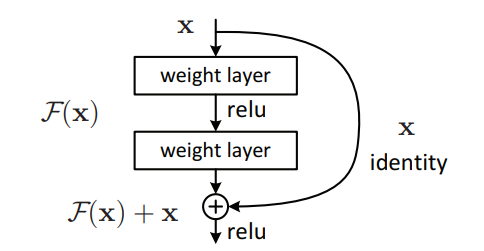
\includegraphics[width=10cm]{./content/materials/residual_orig.png}
    \caption{Cấu trúc của mạng nơ ron nối tắt. Hình ảnh được lấy từ bài báo gốc \cite{residual}}
    \label{fig:residual_net}
\end{figure}

Như vậy, nhằm mục đích tạo ra một mạng tích chập có độ sâu lớn nhưng vẫn đảm bảo mạng không bị tình trạng triệt tiêu đạo hàm, cấu trúc mạng nơ ron nối tắt ra đời. Ý tưởng của mạng nối tắt là sử dụng một đường kết nối để nối tắt qua một hay nhiều lớp tích chập, nhằm đem đặc trưng từ các lớp trước để kết hợp với các đặc trưng sau khi được rút trích bởi mạng tích chập trong khối nối tắt. Kiến trúc này giúp cho mạng được thiết kế sâu hơn mà không phải lo về vấn đề triệt tiêu đạo hàm. Hơn nữa, với kiến trúc này, các lớp sâu phía trong có thêm thông tin từ các lớp ngoài nên sẽ có sự điều chỉnh trọng số hiệu quả hơn. Hình \ref{fig:residual_net} miêu tả kiến trúc của mạng nơ ron nối tắt. Hình \ref{fig:residual_net_in_use} miêu tả chuỗi mạng nơ ron nối tắt được dùng trong bài.

\begin{figure}[H]
    \centering
    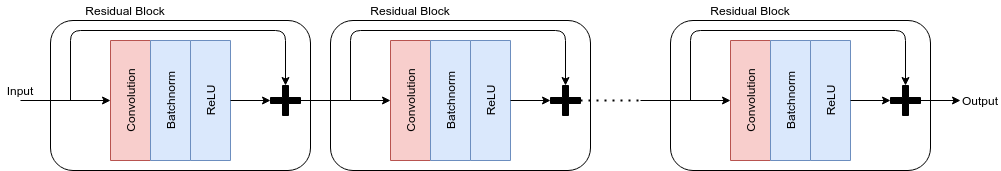
\includegraphics[width=15cm]{./content/materials/residual.png}
    \caption{Mạng nơ ron nối tắt (Residual Network) được dùng trong bài}
    \label{fig:residual_net_in_use}
\end{figure}

% \subsubsection{Các hàm kích hoạt được dùng}

% Trong các mạng học sâu, các lớp có chức năng học như lớp tích chập hay lớp kết nối đầy đủ là những biến đổi tuyến tính trên không gian dữ liệu. Do chúng ta cần phải ghép nối nhiều lớp có chức năng học với nhau để có được một mạng có chiều sâu tương đối, đủ lượng trọng số để học được các đặc trưng của dữ liệu. Tuy nhiên như đã nói, các lớp trên là các lớp tuyến tính, nên việc chồng nhiều lớp tuyến tính lên nhau cuối cùng cũng chỉ tạo ra một phép biến đổi tuyến tính trên không gian dữ liệu. Như vậy, nếu chỉ đơn giản là xếp chồng các lớp tuyến tính lên nhau, mô hình học của mạng sẽ chỉ là một phép biến đổi tuyến tính rất đơn giản và không đủ để tổng quát hóa được những bài toán phức tạp. Vì vậy, ta cần một phép biến đổi phi tuyến để phi tuyến hóa mô hình bài toán. 

% Các hàm kích hoạt là các phép biến đổi phi tuyến được đưa vào mạng nhằm làm cho mạng trở thành một phép biến đổi phi tuyến và có thể mô hình hóa những bài toán phức tạp hơn. Tuy nhiên, hàm kích hoạt cần phải là một hàm phi tuyến có thể đạo hàm được để đảm bảo mạng được cập nhật trọng số ở bước lan truyền ngược.

% \paragraph{Hàm Sigmoid}\mbox{}\\

% Hàm Tanh nhận vào một số thực và trả về giá trị trong khoảng (0, 1). Hàm Sigmoid và đạo hàm của nó được biểu diễn bởi hàm số sau:

% \begin{equation}
% \begin{split}
%     & \sigma(x)=\frac{1}{1+e^{-x}}\\
%     & \sigma'(x)=\sigma(x)*(1-\sigma(x))\\
% \end{split}
% \end{equation}

% \begin{figure}[H]
%     \centering
%     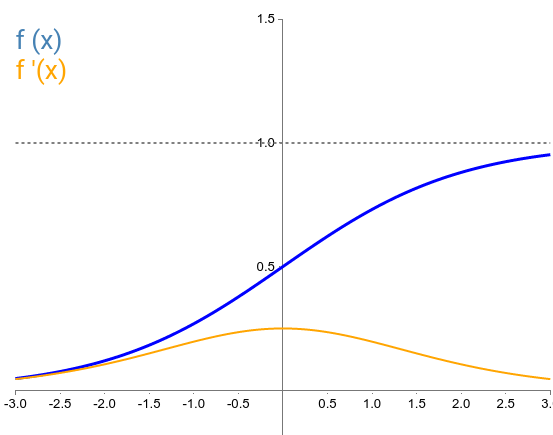
\includegraphics[width=9cm]{./content/materials/sigmoid.png}
%     \caption{Hàm Sigmoid}
% \end{figure}

% Nhìn vào đồ thị của hàm Sigmoid ta thấy, nếu $x$ càng về âm thì $\sigma(x)$ càng tiệm cận về 0 và nếu $x$ càng về dương thì $\sigma(x)$ càng tiến gần đến 1. Tại điểm $x=0$, hàm Sigmoid cho giá trị đạm hàm cực đại và chỉ xấp xỉ bằng 0.3. Với các giá trị đạo hàm khi $x$ càng về âm và càng về dương, đạo hàm của hàm Sigmoid giảm dần về 0. Điểu này gây ra một số bất lợi khi sử dụng Sigmoid để làm hàm kích hoạt:

% \begin{itemize}
%     \item \textbf{Hàm Sigmoid dễ bị bão hòa:} Như đã nói ở trên, đạo hàm của hàm Sigmoid có giá trị gần 0 khi $x$ quá lớn hoặc quá nhỏ. Trong thực tế, nếu mạng nhận được giá trị khởi động rất lớn hoặc rất nhỏ, mạng này sẽ cho ra giá trị cuối cùng cũng rất lớn hoặc rất nhỏ. Trong lúc lan truyền ngược, đạo hàm của nó sẽ đi qua lớp Sigmoid, như ta đã thấy, nếu $x$ rất lớn hoặc rất nhỏ, đạo hàm của Sigmoid sẽ về gần như bằng 0, và trọng số sẽ được cập nhật rất ít, mạng sẽ rất lâu hội tụ.
%     \item \textbf{Hàm Sigmoid dễ bị triệt tiêu đạo hàm:} Ngoài ra, trong trường hợp ngược lại, nếu mạng nhận được trọng số vừa phải, thì lúc này, trong lúc đạo hàm, hàm Sigmoid vẫn cho giá trị đạo hàm rất nhỏ (cao nhất là gần 0.3 tại điểm $x=0$). Nếu sử dụng nhiều lớp Sigmoid trong một mạng học sâu, hiện tượng triệt tiêu đạo hàm sẽ xảy ra.
%     \item \textbf{Hàm Sigmoid không đi qua trục tọa độ:} Vì vậy, việc cập nhật các trọng số  của mạng trong lúc lan truyền ngược sẽ luôn đi theo một hướng cùng dương hoặc cùng âm, làm mất đi sự linh hoạt của việc cập nhật trọng số và làm cho mạng khó hội tụ hơn.
% \end{itemize}

% Trong thực tế, hàm Sigmoid chỉ được sử dụng cho lớp sau cùng của mạng, và được dùng để dự đoán xác suất cho một sự kiện trong bài toán. Nên hạn chế việc sử dụng nhiều lần mạng Sigmoid trên cùng một đường lan truyền vì nó sẽ làm triệt tiêu đạo hàm.

% \paragraph{Hàm Tanh}\mbox{}\\

% Hàm Tanh nhận vào một số thực và trả về giá trị trong khoảng (-1, 1). Hàm Tanh và đạo hàm của nó được biểu diễn bởi hàm số sau:

% \begin{equation}
% \begin{split}
%     & tanh(x)=\frac{e^x-e^{-x}}{e^x+e^{-x}}=2*\sigma(2x)-1\\
%     & tanh'(x)=1-tanh^2(x)\\
% \end{split}
% \end{equation}

% \begin{figure}[H]
%     \centering
%     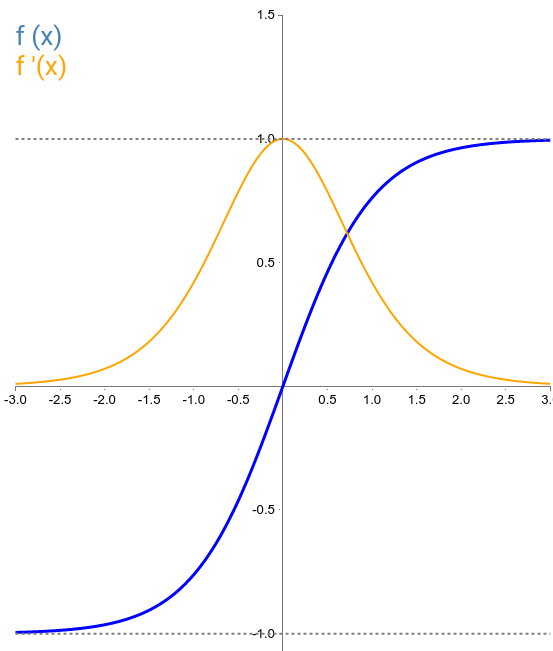
\includegraphics[width=9cm]{./content/materials/tanh.png}
%     \caption{Hàm Tanh}
% \end{figure}

% Nhìn vào đồ thị hàm Thanh ta thấy, hàm Tanh cũng có các tính chất tương tự như hàm Sigmoid: dễ bị bão hòa, dễ bị triệt tiêu đạo hàm. Nhưng nó lại có tính chất đi qua trục tọa độ. Do đó, việc cập nhật trọng số sẽ dễ dàng hơn đối với hàm Tanh. Trên thực tế, giống như hàm Sigmoid, hàm Tanh cũng được dùng để đạt ở những lớp cuối cùng của mạng và cũng không nên đặt nhiều hàm Tanh trên cùng một đường lan truyền để tránh hiện tượng triệt tiêu đạo hàm.

% \paragraph{Hàm điểu chỉnh tuyến tính (Rectified Linear Units - ReLU)}\mbox{}\\

% Hàm điều chỉnh tuyến tính là hàm kích hoạt đơn giản nhưng mang lại hiệu quả cao. Hàm ReLU và đạo hàm của nó được biểu diễn bởi các hàm số sau:

% \begin{equation}
% \begin{split}
%     & f(x) = max(0,x)\\
%     & f'(x) = 
%         \begin{cases}
%             & 1 \text{ if } x>0\\
%             & 0 \text{else}
%         \end{cases}
% \end{split}
% \end{equation}

% \begin{figure}[H]
%     \centering
%     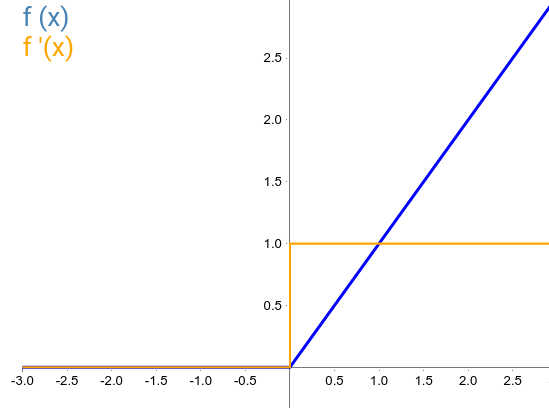
\includegraphics[width=9cm]{./content/materials/relu.png}
%     \caption{Hàm ReLU}
% \end{figure}

% Theo như hàm số trên, ta thấy ReLU chỉ cho phép các giá trị lớn hơn 0 đi qua nó. Như vậy, so với hàm Sigmoid và hàm Tanh, ReLU sẽ không xuất hiện vấn đề triệt tiêu đạo hàm. Đồng thời, việc tính toán cho hàm ReLU cũng diễn ra nhanh hơn đáng kể. Tuy nhiên, ReLU cũng có một nhược điểm là nếu $x$ có giá trị nhỏ hơn 0, nó sẽ được hàm ReLU cho kết quả bằng 0. Vì vậy, giá trị tính toán tại $x$ sẽ không có ý nghĩa cho các lớp tiếp theo, và các hệ số học tương ứng từ đó cũng không được cập nhật trong quá trình lan truyền ngược. Hiện tượng này gọi là \textit{Dying ReLU}.

\section{\texorpdfstring{Cấu trúc mạng tạo sinh đối nghịch (Generative Adversarial Networks - GANs}{gans})}

\subsection{Mạng GANs}\label{sec:base_knowledge_gans}
Vào năm 2014, Ian Goodfellow và cộng sự đã xuất bản một bài báo \cite{gans_base} giới thiệu về mạng tạo sinh đối nghịch (GANs). Mạng GANs đã cho phép máy tính có thể tạo sinh ra dữ liệu chân thật, không phải chỉ bằng một mạng nơ ron, mà là hai mạng nơ ron độc lập. Tuy mạng GANs không phải là mạng nơ ron đầu tiên có chức năng tạo sinh dữ liệu, nhưng kết quả tạo sinh nó mang lại thì có chất lượng vượt xa tất cả các công bố trước đây. Nó đã đạt được những kết quả mà trước đây, người ta không nghĩ là mạng nơ ron học sâu có thể làm được. Mạng GANs có thể tạo sinh hình ảnh giả với độ chân thật cao và có thể so sánh với máy chụp ảnh \cite{gp_gan}, biến những hình vẽ thành ảnh chụp nghệ thuật, hay biến thước phim có hình ảnh của những con ngựa thường thành thước phim có hình ảnh của những con ngựa vằn \cite{cycle_gan}. Và nó làm những điều này mà không cần đến dữ liệu được đánh nhãn.

\begin{figure}[H]
    \centering
    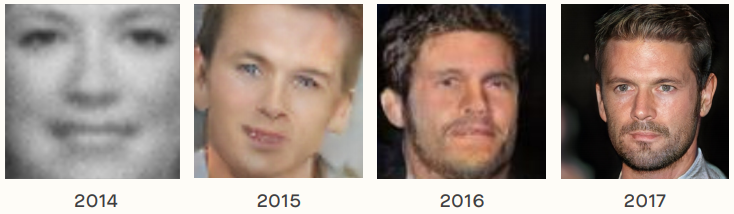
\includegraphics[width=15cm]{./content/materials/gans-faces.png}
    \caption{Việc tạo sinh mặt người dùng mạng GANs qua các năm \cite{gans_faces}}
\end{figure}

Mạng tạo sinh đối nghịch (GANs) là một loại mạng thần kinh học sâu dùng để tạo sinh dữ liệu tùy theo mục đích của người sử dụng dựa trên những tri thức mà nó được học từ dữ liệu mẫu. Mạng tạo sinh đối nghịch bao gồm hai mạng nhỏ hơn là mạng tạo sinh (Generator) và mạng phân biệt (Discriminator). Mạng tạo sinh được huấn luyện để sinh ra dữ liệu mới, trong khi mạng phân biệt được huấn luyện để phân biệt dữ liệu nào là dữ liệu thật được lấy từ tập dữ liệu huấn luyện, dữ liệu nào là dữ liệu giả được sinh ra bởi mạng tạo sinh. Ví dụ, chúng ta muốn tạo sinh các bức họa có phong cách vẽ giống với Leonardo da Vinci, ta có thể dùng tập dữ liệu các bộ tranh vẽ của Leonardo da Vinci để huấn luyện cho mạng. Mạng tạo sinh sẽ cố gắng học cách tạo sinh ra các bức họa giống với phong cách của Leonardo da Vinci nhất, trong khi mạng phân biệt cố  học cách phân biệt các bức họa thật giả, với ảnh thật là các ảnh lấy trực tiếp từ dữ liệu huấn luyện, còn ảnh giả là các bức ảnh được tạo ra bởi mạng tạo sinh.

\subsection{Cách hoạt động của mạng GANs}
\begin{figure}[H]
    \centering
    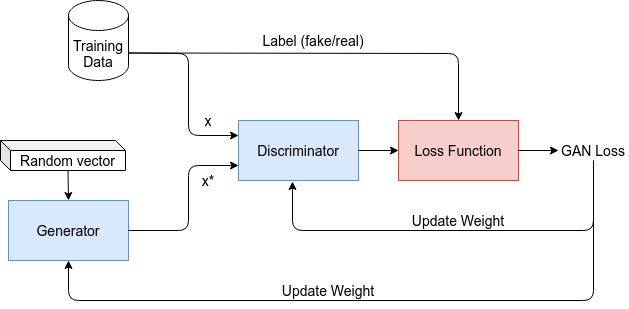
\includegraphics[width=15cm]{./content/materials/gans-pure.png}
    \caption{Cấu trúc mạng GANs thông thường}
    \label{fig:pure-gans}
\end{figure}

Như vậy, mục đích của mạng tạo sinh là tạo ra những dữ liệu có cùng tính chất với dữ liệu được đưa vào để huấn luyện cho nó, những dữ liệu được sinh ra phải chân thật đến nỗi không thể phân biệt được với dữ liệu thật. Mạng tạo sinh có thể được xem như một phiên bản ngược của mạng nhận diện (Object Recognition Networks). Trong khi mạng nhận diện có chức năng học những chi tiết, đặc trưng trên những tấm ảnh nó được học qua để tìm ra được vật thể trên ảnh. Thì với mạng tạo sinh, thay vì học các chi tiết, đặc trưng của vật thể, nó học cách để tạo ra các chi tiết, đặc trưng đó với đầu vào chỉ đơn giản là một vec tơ được tạo sinh ngẫu nhiên bằng phân phối chuẩn (đói với mạng GANs truyền thống). 

Việc học cách tạo sinh dữ liệu được mạng tạo sinh thực hiện nhờ vào phản hồi của mạng phân biệt Discriminator. Mục đích của mạng phân biệt là tìm cách phân biệt dữ liệu đầu vào cũa nó, dữ liệu nào được tạo sinh và dữ liệu nào là dữ liệu thật. Do vậy, mỗi lần mạng phân biệt bị đánh lừa bởi mạng tạo sinh (nhận nhầm dữ liệu tạo sinh là dữ liệu thật), mạng tạo sinh biết là nó đang làm đúng. Và ngược lại, mỗi lần mạng phân biệt bắt được đúng dữ liệu giả, thông tin này sẽ được đưa về cho mạng tạo sinh và nó sẽ phải cập nhật lại trọng số để tạo sinh dữ liệu chân thật hơn.

Mạng phân biệt cũng dần được cải thiện qua mỗi lần nó phân biệt sai dữ liệu. Với hàm mất mát Binary Cross Entropy, nó tính toán được khoảng cách từ dự đoán của chính nó đến kết quả thực và từ đó thay đổi trọng số của mạng để dự đoán của nó ngày càng phù hợp hơn với phân phối dữ liệu. Cứ như vậy, mạng tạo sinh càng ngày càng sinh ra dữ liệu chân thực hơn nhằm mục đích đánh lừa mạng phân biệt, nhưng mạng phân biệt cũng ngày càng trở nên tốt hơn trong việc phân biệt dữ liệu thật - giả.

\subsection{Huấn luyện mạng GANs}

Do mạng GANs là tổng hợp của hai mạng tạo sinh và mạng phân biệt, nên cách huấn luyện mạng cũng có sự khác biệt so với các loại mạng khác. Khi huấn luyện mạng GANs, ta sẽ đi huấn luyện cho cả hai mạng tạo sinh và phân biệt cùng một lúc. Chi tiết các bước huấn luyện một mạng GANs truyền thống được miêu tả ở Hình \ref{fig:pure-gans} như sau:

Với mỗi lượt huấn luyện, ta lần lượt thực hiện:
\begin{itemize}
    \item Huấn luyện mạng phân biệt:
    \begin{itemize}
        \item Lấy một vài mẫu dữ liệu thật ($x$) từ tập dữ liệu huấn luyện
        \item Lấy mẫu ngẫu nhiên dựa trên phân phối chuẩn để tạo ra véc tơ $z$, đưa véc tơ $z$ vào mạng tạo sinh để tạo ra dữ liệu giả ($x^*$)
        \item Sử dụng mạng phân biệt để phân biệt $x$ và $x^*$
        \item Tính toán hàm mất mát của mạng phân biệt và thực hiện lan truyền ngược trên mạng phân biệt nhằm tối thiểu hóa hàm mất mát
    \end{itemize}

    \item Huấn luyện mạng tạo sinh:
    \begin{itemize}
        \item Lấy mẫu ngẫu nhiên dựa trên phân phối chuẩn để tạo ra véc tơ $z$, đưa véc tơ $z$ vào mạng tạo sinh để tạo ra dữ liệu giả ($x^*$)
        \item Sử dụng mạng phân biệt để phân biệt dữ liệu giả vừa được tạo sinh
        \item Tính toán hàm mất mát của mạng phân biệt và thực hiện lan truyền ngược trên mạng tạo sinh nhằm tối đa hóa hàm mất mát
    \end{itemize}
\end{itemize}

\subsection{Điểm cân bằng trong huấn luyện mạng GANs}

Vậy khi nào thì việc huấn luyện mạng GANs nên được dừng lại? Làm sao và dựa vào dấu hiệu nào để biết được mạng GANs đã hội tụ? Với các mạng nơ ron thông thường khác, ta thường có các thông số rõ ràng và những mục tiêu rõ ràng để biết khi nào thì dừng việc huấn luyện. Ví dụ như với mạng phân lớp, ta có thể chia dữ liệu huấn luyện thành tập để học và tập để kiểm thử. Khi giá trị hàm mất mát trên tập kiểm thử bắt đầu tệ đi là lúc ta nên dừng quá trình huấn luyện mạng vì mạng đã bắt đầu học thuộc dữ liệu. Trong mạng GANs, hai mạng tạo sinh và phân biệt có hai mục tiêu trái ngược nhau. Bên tạo sinh cố gắng tạo ra dữ liệu thật chân thật để đánh lừa bên phân biệt, trong khi bên phân biệt ngày càng cải thiện bản thân để phân biệt thật - giả tốt hơn. Như vậy, nếu bên tạo sinh có giá trị hàm mất mát thấp hơn, thì giá trị hàm mất mát của bên phân biệt sẽ cao lên và ngược lại.

Như vậy, ta có thể thấy đây là một trò chơi có tổng bằng 0 (zero-sum game), ở đó, bên này được bao nhiêu thì bên kia mất bấy nhiêu. Tất cả mọi zero-sum game đều có một điểm cân bằng Nash (Nash equilibrium) mà tại đó, cả hai bên đều không thể làm gì để cải thiện tình hình chung. Mạng GANs đạt được trạng thái cân bằng Nash khi những điều kiện sau đây được thỏa mãn:
\begin{itemize}
    \item Mạng tạo sinh có thể tạo ra dữ liệu giả không thể phân biệt được với dữ liệu thật
    \item Mạng phân biệt có thể dự đoán một cách ngẫu nhiên một mẫu dữ liệu là thật hay giả (độ chính xác của bộ phân biệt đạt 50\%)
\end{itemize}
Khi trạng thái này xảy ra, mạng phân biệt không còn khả năng để dự đoán mẫu dữ liệu nào là thật, mẫu dữ liệu nào là giả, vì vậy nó không thể giúp ích gì thêm cho mạng tạo sinh nữa. Mạng tạo sinh cũng không còn khả năng cải thiện hơn, vì dữ liệu nó sinh ra đã không còn có thể được nhận diện bởi mạng phân biệt. Vì vậy, khi ở trạng thái này, mạng GANs đã hội tụ và ta có thể ngừng việc huấn luyện tại đây.

Nhưng trên thực tế, trạng thái cân bằng Nash dường như không thể đạt được bởi sự phức tạp và rộng lớn của không gian dữ liệu, với số chiều rất lớn và là tập hợp của các hàm tuyến tính, hàm kích hoạt, lấy mẫu, và đôi khi là hàm xác suất,... tất cả những hàm đó tạo nên một không gian không lồ, và với việc sử dụng các giải thuật tối ưu như SGD và Adam, đôi khi ta chỉ tìm được các điểm tối ưu cục bộ. Trên thực tế, sự hội tụ của mạng GANs vẫn còn là một câu hỏi mở cho ngành trí tuệ nhân tạo.

\subsection{\texorpdfstring{Đặc trưng MFCC (mel-frequency cepstrum coefficients) của dữ liệu âm thanh}{mfcc}}\label{sec:base_knowledge_mfcc}

Đầu tiên, ta sẽ đi qua định nghĩa về cepstrum. Cepstrum là một đặc trưng quan trọng để phân biệt các nguyên âm trong xử lý tiếng nói. Về mặt ý nghĩa, cepstrum giúp phân biệt các nguyên âm do nó là đặc trưng được sinh ra từ tần số của âm thanh. Khi con người cất tiếng nói, một nguyên âm nào đó khi phát ra sẽ được cuốn họng rung để tạo ra tần số cơ bản, khoang mũi, miệng, lưỡi và môi giống như các bộ lọc âm thanh để tạo ra các tần số mới, và các đỉnh cực đại của các tần số khác nhau trong tín hiệu tiếng nói quyết định âm được nói ra là âm gì. Để chuyển sự biểu diễn âm thanh từ miền thời gian sang miền tần số, người ta thường dùng biến đổi Fourier. Một âm thanh tiếng nói khi được biến đổi Fourier sẽ tạo ra một hàm số thể hiện biên độ của các tần số khác nhau. Đồ thị này sẽ có các điểm cực đại, và các điểm cực đại này là đặc trưng cho nguyên âm vừa được nói ra (như đã nói ở trên). Khi hàm biến đổi Fourier này được đưa về dạng hàm trơn, ta gọi đó là cepstrum. Các nguyên âm khác nhau thì mỗi nguyên âm sẽ có một dạng biểu diễn đồ thị cepstrum khác nhau, phân biệt khá rõ ràng về số đỉnh và khoảng cách giữa các đỉnh.

Tai của con người có một đặc điểm quan trọng, chúng hoạt động như những bộ lọc âm thanh, nhạy cảm hơn với các âm ở tần số thấp và ít nhạy hơn với âm thanh ở tần số cao. Vì vậy, bộ lọc Mel ra đời nhằm xử lý các âm thanh tiếng nói để trích xuất các đặc trưng sao cho phù hợp với cách nghe của con người. Theo đó, các giá trị tần số nhỏ hơn 1kHz sẽ được lọc với bộ lọc tuyến tính, điều này phù hợp với lý thuyết là tai người nhạy cảm với âm thanh có tần số thấp. Dải tần số trên 1kHz được lọc với bộ lọc phi tuyến và bộ lọc thưa dần khi lên đến các tần số cao hơn.

MFCC là một đặc trưng âm thanh và được tạo ra nhằm mục đích duy nhất là dùng cho giọng nói con người. Vì vậy, MFCC thường được sử dụng trong các bài toán nhận dạng giọng nói hay phân loại giọng nói. MFCC sẽ cho ra kết quả là các hệ số của cepstrum được lấy từ bộ lọc Mel sau khi xử lý phổ của âm thanh giọng nói.
